\documentclass{article}

\usepackage[inline]{enumitem}
\usepackage{amsmath}
\usepackage{graphicx}

\newcommand{\ds}{\displaystyle}

\begin{document}

\noindent{}\rule{\textwidth}{0.4pt}
\begin{center}
	Universidade Federal da Grande Dourados\\
	An\'alise Num\'erica --- Lista 3 \\
	Engenharia Mec\^anica --- 2016.2 \\
	Prof.\ Adriano Barbosa
\end{center}
\noindent{}\rule{\textwidth}{0.4pt}

\begin{enumerate}
	\item Use o m\'etodo de Horner para avaliar os polin\^omios utilizando
		aritm\'etica computacional de 3 d\'{\i}tigos e arredondamento:
		\begin{enumerate}
			\item $f(x) = x^3 -2x^2 -5$, $f(0.25)$
			\item $f(x) = x^3 - x - 1$, $f(\sqrt{2})$
			\item $f(x) = x^5 - x^4 + 2x^3 - 3x^2 + x - 4$, $f(\pi)$
		\end{enumerate}

	\item Avalie $f'(x)$ para cada $f(x)$ na primeira quest\~ao nos pontos dados.

	\item Avalie os polin\^omios da primeira quest\~ao diretamente usando
		aritm\'etica computacional de 3 d\'{\i}gitos e arredondamento. Compare os
		resultados com o resultado exato.

	\item Utilize o m\'etodo de Newton para encontrar as ra\'{\i}zes e os pontos
		cr\'{\i}ticos das fun\c{c}\~oes polin\^omiais abaixo. Use essa informa\c{c}\~ao para
		esbo\c{c}ar o gr\'aficos das fun\c{c}\~oes.
		\begin{enumerate}
			\item $f(x) = x³ - 9x^2 + 12$
			\item $f(x) = x^4 - 2x^3 - 5x^2 + 12x + 5$
		\end{enumerate}

\end{enumerate}

Respostas:

\noindent{}1. (a) $-5.109$ (b) $0.4$ (c) $240$

\noindent{}2. (a) $-0.813$ (b) $4.97$ (c) $405$

\noindent{}3. (a) $6.24$ (b) $0.4$ (c) $240$

\noindent{}4. 
\begin{figure}[!h]
	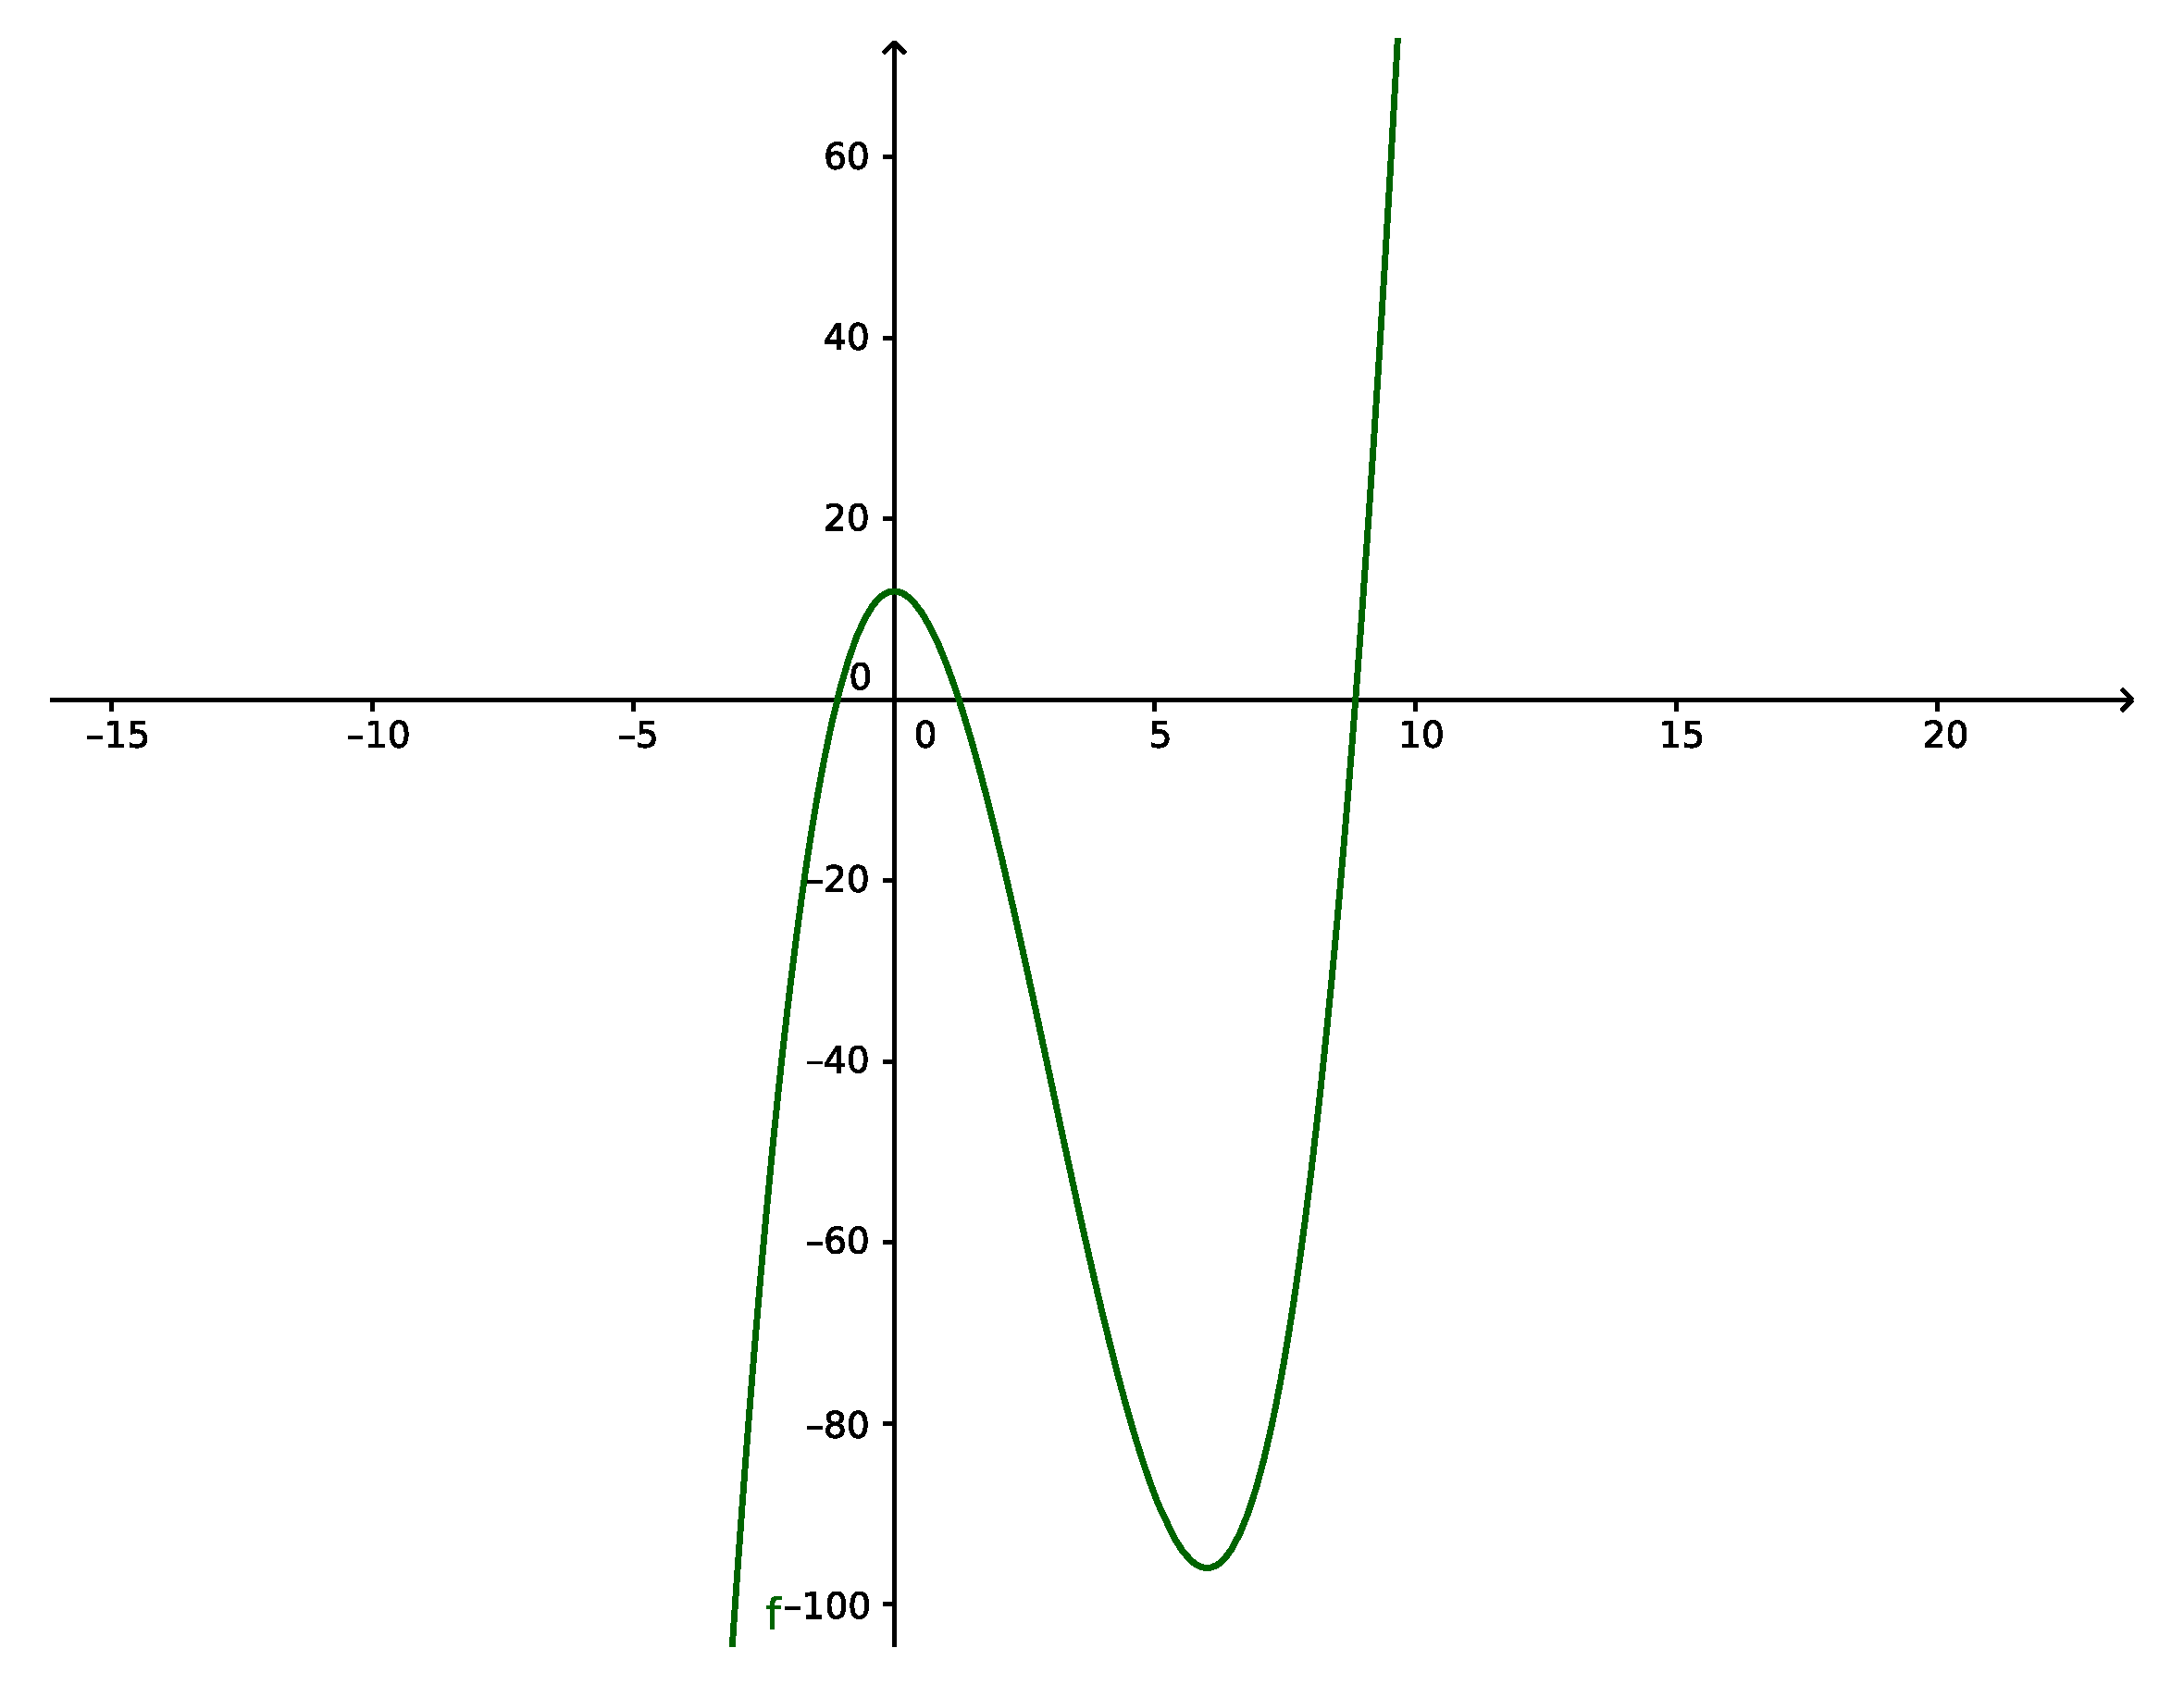
\includegraphics[width=0.5\textwidth]{a.pdf}
	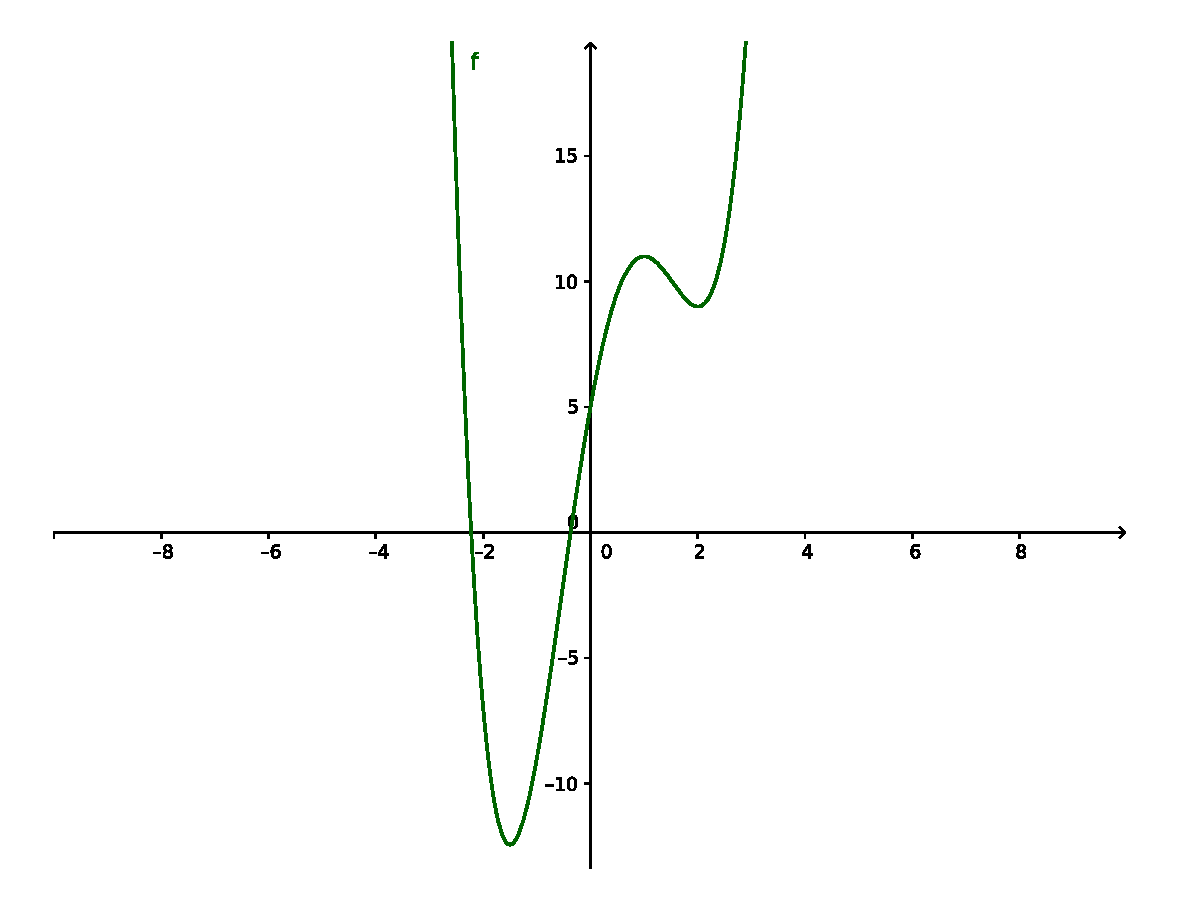
\includegraphics[width=0.5\textwidth]{b.pdf}
\end{figure}
\newpage{}

\end{document}  % chktex 16
